%\Fix{NK: I think that this section should be titled ``Overview'' and should start with a paragraph that defines what a ``session'' (or ``comprehension session'') is and provides a high-level description of how code smells and comprehension cost fit in (and relate to principal and interest).}

%Within the proposed framework, we consider \TD to be dependent on the maintenance and evolution activity in the code base, meeting the criteria that \TD could result from a context shift requiring stable code to be revised~\cite{Ozkaya_etal:2012}.
The framework we propose combines related metrics from code structure and code comprehension data sources.  We selected some relevant code structure metrics related to maintainability and \TD using work by Nugroho et al.~\cite{Nugroho_etal:2011}, in which potential code maintainability issues are identified using static code metrics.  We use some of the class-level static code metrics provided by $Understand$.\footnote{\url{http://www.scitools.com}} to identify code that may have maintainability concerns related to effort required to comprehend the code. In particular, the framework uses the following metrics:
\newpage
\begin{description}[font=\itshape\mdseries,leftmargin=.42\linewidth,style=sameline]
    \item[Count Class Coupled] number of other classes coupled to
    \item[Count Class Base] number of immediate base classes
    \item[Count Class Derived] number of immediate sub-classes
    \item[Count Line Code] number of lines in the class
    \item[Count Declared Method] number of local methods in the class
\end{description}

These class-level code-structure metrics relate to the comprehension metrics on which we based interest estimation. We define low-level code comprehension metrics based on developer actions as they work on code inside of or related to a class.

Data for calculating developer comprehension metrics comes from the $Blaze$~\cite{Snipes_etal:2014} monitoring tool.  $Blaze$ anonymously logs developer actions in Visual Studio, including uses of menu commands, shortcut keys, and navigation commands (such as moving the insertion caret and scrolling).  Developers at ABB volunteered to install $Blaze$ and to have their actions recorded.  The data set we used for the initial study in this paper includes data from two developers that spans over 3 months.

Table~\ref{fig:SampleEventData} shows a sample of the log data, where each row contains the date (not shown) and time for an action, the unique ID for the developer who performed the action, the name of the action that was performed, and the name of and line in the file in which the action occurred.

\begin{table}[!t]
    \renewcommand{\arraystretch}{1.3}
    \centering
    \caption{Sample Data From Event Log}
    \begin{tabular}{llll}
        \toprule
        \textbf{Time-stamp} & \textbf{User} & \textbf{Event} & \textbf{Artifact} \\
        \midrule
        22:04:51 & N3 & View.SourceFile & 1acc7366.cs/10 \\
        22:04:52 & N3 & View.OnChangeCaretLine & 1acc7366.cs/14 \\
        22:04:53 & N3 & View.OnChangeCaretLine & 1acc7366.cs/16 \\
        22:04:58 & N3 & Menu.ViewCallHierarchy & 1acc7366.cs/16 \\
        22:05:00 & N3 & View.OnChangeCaretLine & 1acc7366.cs/20 \\
        22:05:19 & N3 & View.SourceFile & 81c2db1a.cs/1 \\
        22:05:22 & N3 & Edit.Find & 81c2db1a.cs/1 \\
        22:05:30 & N3 & Edit.FindNext & 81c2db1a.cs/20 \\
        \bottomrule
    \end{tabular}
    %	\includegraphics[width=2.75in]{figures/SampleEventData.pdf}
    \label{fig:SampleEventData}
\end{table}

Our approach to analyzing the developer activity data was to establish sessions that segment the stream of activity into periods in which the developer is focused on a particular class. We define a session as fixed length time window where the developer is investigating a certain class that we call the central class.  The session time window begins the first time a developer visits a particular class and ends with the last time the developer visits that class within a fixed length time window. The length of the time window is a variable that we investigate in Section \ref{sec:AnalysisResults}.  

Figure \ref{fig:SessionDataConcept} illustrates the session concept.  The session starts with the first visit to Class A under the green circle.  After that, other classes C and E are visited, including a visit to Class A again before the last visit to Class A under the red hexagon.  After the last visit, the session time window expires (assuming a fixed-time window).  The second session starts with a visit to Class A.  In this session, classes C and E are visited before the developer returns to Class A.  Thus, there are two sessions for Class A, in which there are a total of five visits to Class A, three visits to Class C, and two visits to Class E.

\begin{figure}
    \centering
    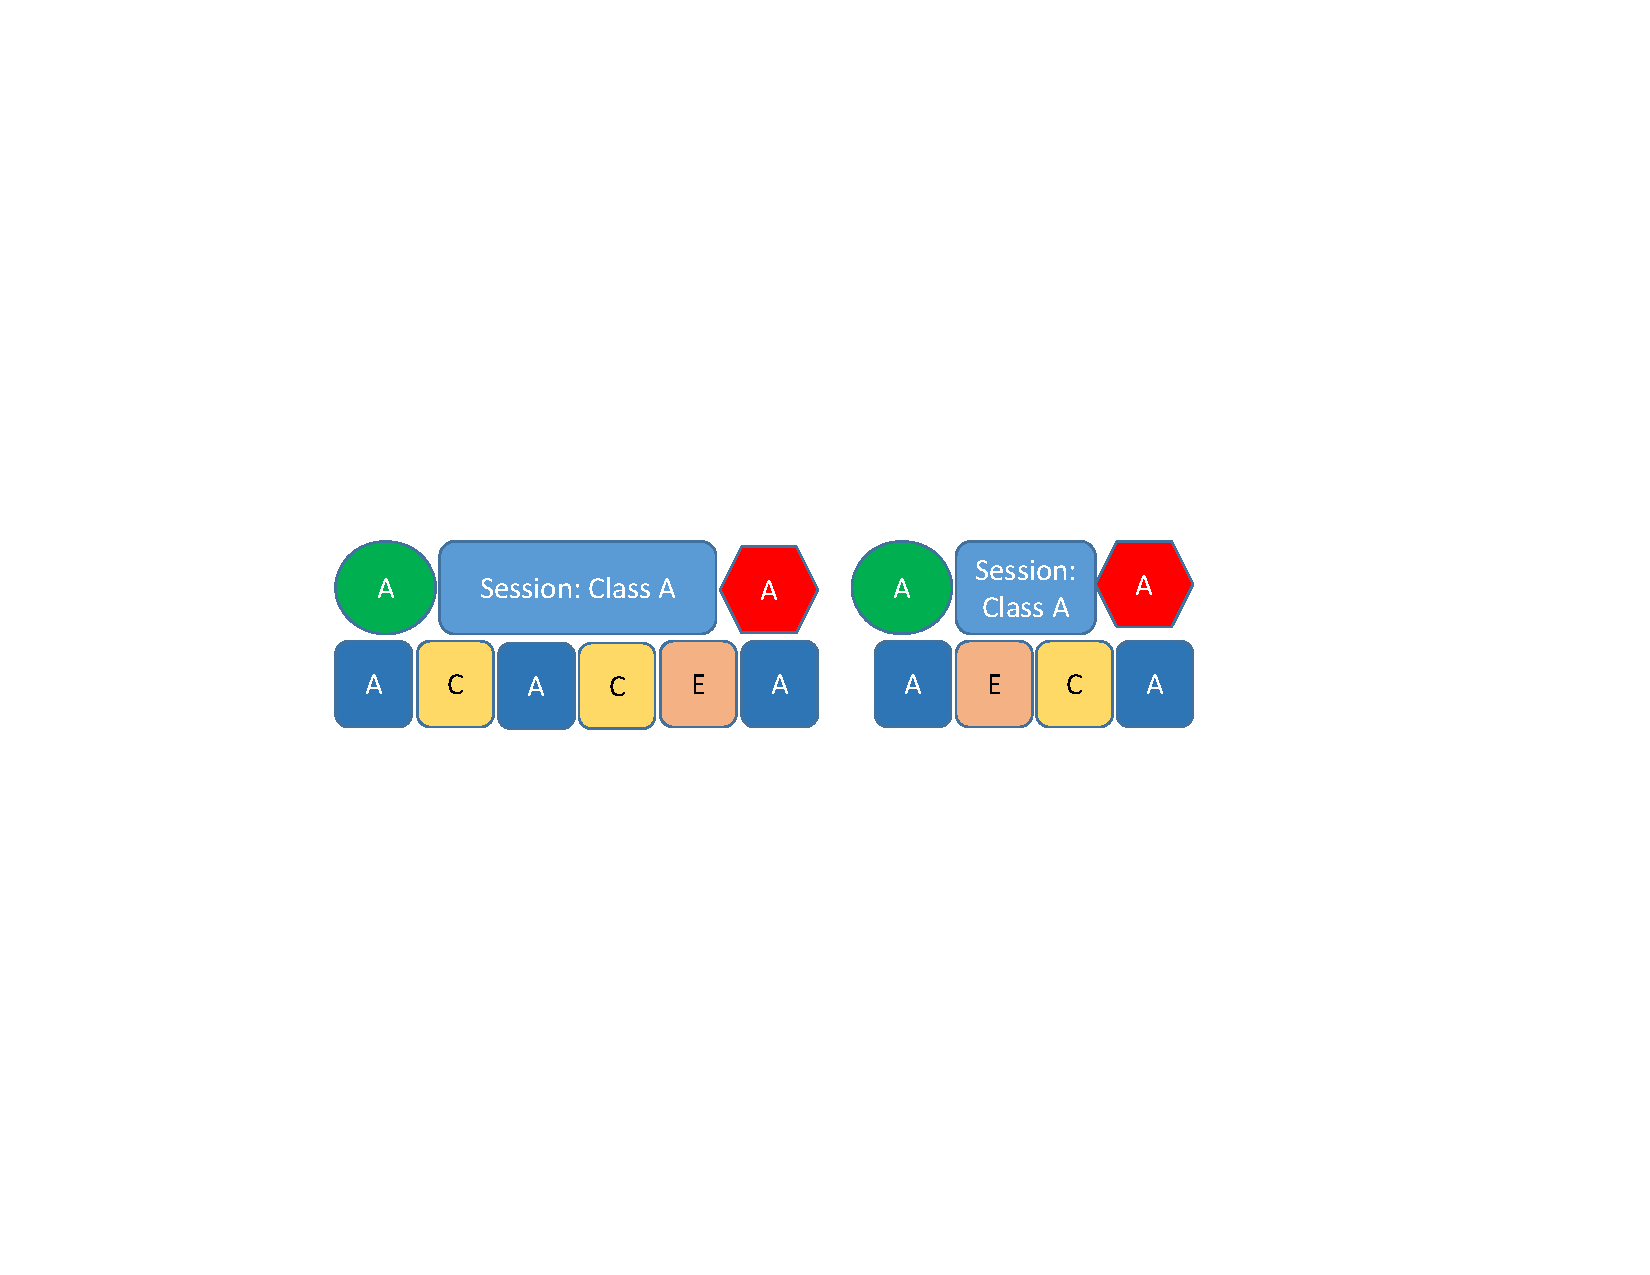
\includegraphics[width=.66\linewidth]{SessionDataConcept.pdf}
    \caption{Conceptual View of Sessions}
    \label{fig:SessionDataConcept}
\end{figure}

%\Fix{The following is unclear in the context of block and super block}
%When there are multiple sessions for a class, the sessions may involve visits to different sets of other classes. Regardless, they incur some comprehension effort which we add to the interest payments.  For each session we determine the interest payment from the comprehension data quantifying it in hours. 

Within a session, we calculate metrics related to comprehension effort as follows:
\begin{description}[font=\itshape\mdseries,style=nextline]
    \item[\#~Sessions] number of time-window sessions for each class 
    \item[\#~Class~Visits] number of times the central class is visited in a session
    \item[\#~Other~Class~Accesses] number of unique (non-central) classes visited in a session
    \item[Time~Spent~in~Class] time spent in the central class for a session
    \item[Time~Spent~in~Other~Classes] time spent in all other classes in a session
\end{description}

The class-level metrics for code structure are related to comprehension metrics through the name of the source file in the $Blaze$ data corresponding to the class.  In cases where the source file contains multiple classes, the structure metrics were aggregated.


We can investigate how much the Feature Envy smell  where a method makes too many calls to other classes to obtain data or functionality.  We assess the level of Feature Envy using using the $Class Coupled$ static metric and quantify the effect that has on comprehension using the $\# Other Class Accesses$ metric and evaluate the effort this smell generates using the $Time Spent in Other Classes$ measure.  
%We can estimate the level of Shotgun Surgery performed by measuring $Count Class Coupled$ and $Count Class Derived$ combined with the comprehension data of $\# Other Class Accesses$ and $Time Spent in Other Classes$.  
We can estimate the impact of the Large Class smell, where a class is larger than typical, by using the $Count Line Code$ static metric.  The assess the effect on developer comprehension, we can use the metrics $\# Class Visits$, $\# Sessions$ to determine the difference in navigation behavior and evaluate the $Time Spent in Class$ to assess the total effort resulting from the smell.

By defining the measurement framework, the calculation of interest payments on \TD related to code structure will use time spent measurements for classes with static metrics that indicate code is difficult to maintain or contains smells.  Thus static metrics will indicate the possible presence of \TD in a class and comprehension effort metrics will quantify the effort to comprehend those classes. The study of correlation between static metrics and comprehension effort is planned for future research.

%\begin{itemize}
%    \item[] How much time does the developer spend understanding the code related to the change they are making?
%    \item[] How many code elements does the developer need to review related to the change?
%    \item[] How many dependent classes does the developer need to review related to the change?
%    \item[] How correlated are comprehension effort metrics with code structure metrics?
%    \item[] As code-structure metric values change, is the corresponding change in comprehension effort linear or non-linear.
%\end{itemize}


%The comprehension effort relates to \TD through occurrence of code smells in one dimension.  For example, consider the code smell of Feature Envy where a method makes too many calls to other classes to obtain data or functionality.  By calculating from $Blaze$ data the number \Fix{NK: The number of what?} and time spent visiting other classes within a session \Fix{The concept of a session needs to be introduced/defined in the previous paragraph}, we can estimate the developer effort required to understand dependencies.  The total count of visits to other classes relates to the Feature Envy smell or Inappropriate Intimacy. Further, the number of (unique) classes visited in each session could  relate to the Shotgun Surgery smell, particularly when multiple classes are edited in a session. The time spent visiting classes and time per class visited may relate to the Long Class smell~\cite{Fowler_etal:1999}.  

%\Fix{Will: wording this next phrase}
%In order to confirm the above idea, we collect source code metrics from the code being viewed and edited by the developers.  .